\scanpage{320}
\[
\diagram{\begin{tikzcd}
\deleted{\unsure{F_A}(\Gamma^{pq}(X))}\arrow[r]&{}
\end{tikzcd}}
\]
\margin{$\Gamma^{pq}(f)\circ u_{pq}$}
\[
\diagram{\begin{tikzcd}[column sep=large,row sep=large]
\Gamma^{pq}(F_A(X))\arrow[r,"\sigma_{pq}^X"]\arrow[d]&F_A(\Gamma^{pq}(X))&{}\\
\Gamma^p(\Gamma^q(F_A(X)))\arrow[r,"\Gamma^p(\sigma_q^X)"]&\Gamma^p F_A\Gamma^q(X)\arrow[r]&F_A(\Gamma^p\Gamma^q(X))
\end{tikzcd}}
\]
\inserted{$\unsure{f^{pq}}$}
\margin{$f^{\unsure{(pq)|(rs)}}\in$}
\margin{$(f^{(q)})^{(p)}$}
\inserted{$(\Gamma^q(f)\circ u_q)^{(p)}$}
\deleted{$\unsure{F_A\Gamma^p(\Gamma^q(X))}$}
\margin{$F_A(\sigma_{p,q}^X)$}
\margin{$(\sigma_{pq}^X\circ\Gamma^{pq}(f)\circ u_{pq})$}
\figure{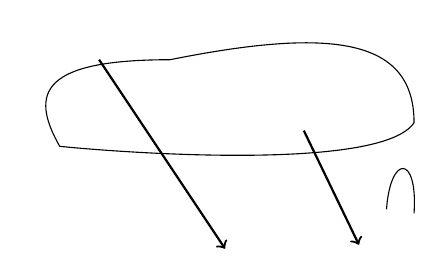
\begin{tikzpicture}
\draw (0,0) .. controls (-.4,.7) and (-.2,1.1) .. (1.4,1.1) .. controls (3.4,1.5) and (4.5,1.4) .. (4.5,.3) .. controls (4.1,-.3) and (1,-.1) .. (0,0);
\draw[->,thick] (.5,1.1)--(2.1,-1.3);
\draw[->,thick] (3.1,.2)--(3.8,-1.25);
\draw (4.15,-.8) .. controls (4.2,-.1) and (4.55,-.1) .. (4.5,-.85);
\end{tikzpicture}}
\inserted{$\Gamma^p(\Gamma^q(f)\circ u_q)\circ u_p$}

\[
\diagram{\begin{tikzcd}[column sep=large,row sep=large]
\unsure{A'|A}\arrow[r,"u_{pq}"]\arrow[dd,"u_p"']&\Gamma^{pq}(A)\arrow[r,"\Gamma^{pq}(f)"]&\Gamma^{pq}(X)\arrow[d,"\sigma_{pq}^X"]\\
{}&{}&\Gamma^p(\Gamma^q(X))\\
\Gamma^p(A)\arrow[r,"\Gamma^p(u_q)"']\arrow[urr,bend left=12]&\Gamma^p(\Gamma^q(A))\arrow[ur]\arrow[r,draw=none,"\deleted{\longrightarrow}" description]&\deleted{\unsure{\Gamma^p(\Gamma}}\vphantom{\Gamma^q(A)}
\end{tikzcd}}
\]
\inserted{$\Gamma^p(\Gamma^q(f))$}
\deleted{$\unsure{\longrightarrow}$}
\margin{$f:A\longrightarrow X$}
\margin{$\Gamma^q f:\Gamma^q A\longrightarrow\Gamma^q X$}
\margin{$\Gamma^q f\circ u_q$}
\[
\diagram{\begin{tikzcd}
{}&\unsure{u_q}\\
A\arrow[ur,no head]&{}
\end{tikzcd}}
\]

$X=A,\ f=\mathrm{id}_A$
\[
\diagram{\begin{tikzcd}[column sep=large,row sep=large,execute at end picture={\draw (current bounding box.center) ellipse [x radius=3.8cm,y radius=2cm];}]
A\arrow[r,"u_{pq}"]\arrow[d,"u_p"']&\Gamma^{pq}(A)\arrow[d,"\sigma_{pq}^A"]\\
\Gamma^p(A)\arrow[r,"\Gamma^p(u_q)"']&\Gamma^p(\Gamma^q(A))
\end{tikzcd}}
\]
\figure{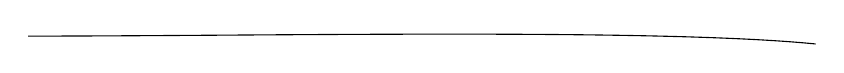
\begin{tikzpicture}\draw (0,0)..controls(3,0)and(8,.1)..(10,-.1);\end{tikzpicture}}

\[
\diagram{\begin{tikzcd}[column sep=large,row sep=large]
A\otimes A\arrow[r,"u_p\otimes u_q"]&\Gamma^p(A)\otimes\Gamma^q(A)\arrow[d,"\unsure{\beta_{p,q}^A}"]\\
A\arrow[u,"\Delta"]\arrow[r,"\unsure{c_{pq}|\gamma_{pq}}u_{p+q}"']&\Gamma^{p+q}(A)
\end{tikzcd}}
\]
\margin{$h\{T\}$}
\figure{\begin{tikzpicture}\draw[->] (.6,.7)--(0,0);\end{tikzpicture}}
\[
\boxed{u_p.u_q=\unsure{c_{pq}|\gamma_{pq}}u_{p+q}}\quad\text{dans }\operatorname{Hom}_{\unsure{1}}(A,\Gamma^*A)\simeq\unsure{(\operatorname{H}_{-},\mathrm{S}_\gamma\check A,\check A)}
\]
qui est une alg. grâce à la structure de coalg. sur $A$ et la structure d’alg. de $\Gamma^*A$
\[
\boxed{u_o=1}\qquad\boxed{u_1=\mathrm{id}}
\]
\figure{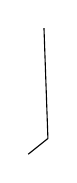
\begin{tikzpicture}\draw (0,.8)--(.05,-.6)--(-.2,-.8);\end{tikzpicture}}
\margin{321}
